\documentclass{article}

% Language setting
% Replace `english' with e.g. `spanish' to change the document language


% Set page size and margins
% Replace `letterpaper' with `a4paper' for UK/EU standard size
\usepackage{geometry}
 \geometry{
 a4paper,
 total={170mm,257mm},
 left=20mm,
 top=20mm,
 }
  \usepackage{ifthen}
  \usepackage{array}
     \setlength{\extrarowheight}{2pt}
    \newcounter{rowcount}
\usepackage{graphicx}
\graphicspath{ {./images/} }

\usepackage{float}
 
%Packages
%Coloums

\usepackage{multicol}
\usepackage{tabularx}
\usepackage{amsmath}
\usepackage[colorlinks=true, allcolors=blue]{hyperref}
\usepackage{titlesec}

\title{Software Requirements Specification(SRS)}
\author{The Great UNKNOWN}

\begin{document}

\maketitle

\tableofcontents

\pagebreak


\section{Client Brief}

The client brief has been based upon a questionnaire produced by a company called "The Great UNKNOWN"  a copy of which is attached at Appendix A.
\\
\\
The website will consist of six components:  homepage; login/join page; book your journey; about us; pictures of use; and user account management page

\subsection{Home Page}
The homepage is the first page that our customers will see when they open the website. It must include pictures of previous voyages and advances in our space technology. Text will be interleaved between the photos or on top of the pictures to show why customers should spend their money on a trip with the client. There will be a static navbar with links to the other pages on the site, there will also be a footer with a navbar with links to other information e.g. financial reports, history, Terms of Service (ToS) etc.

\subsection{Login/Join Page}
The Login Page must be simple and straightforward. It will contain a box with a username, password and name and a sign up login button. After the customer has logged in they will be requested to add their billing address and bank details. When they have completed the setup they will be redirected to the Book Your Journey page.

\subsection{User Account Management Page}
The User Account Management Page (U.A.M) has to include a section to allow the customer's billing address, bank details, password and usernames to be amended and their account deleted. 

\subsection{Book Your Journey}
This page should be seamless for the user. When they open the page they will be immediately presented with a list of journeys that are currently available. The page will include a table which will be organised as a calendar, the month will be shown at the top and below that to the left will be the days. Time slots will be included to the right, with small red dots in the middle indicating availability. 

\subsection{Pictures of us}
The Pictures page will be minimalist in design, little or no words will be included, just the minimum necessary to describe the image. The layout of the page will have one image following another in a square like pattern, with boxes varying in size depending on size and importance of image. Using images will hopefully entice the user to be part of our journey and explore what is beyond our small plant that we call home.

\subsection{About us}
The About Us page the is the most sensible page of all. It will include all the legal documents showing the necessary  certificates that prove we are certified to fly these ships. It will explain our ethos, who we are and why we want to take you in to space. It will have all our copyrights, trademarks and patents so no one can copy our ships and steal our designs.

%\bibliographystyle{alpha}
%\bibliography{sample}
\pagebreak


\section{Graphs}

\subsection{Entity Relationship Diagram}
\begin{figure}[htbp]
    \includegraphics[width=0.85\linewidth]{{NERD.png}}
    \caption{This is our Friendly NERD}
    \label{fig:NERD}
\end{figure}

Figure ~\ref{fig:NERD} above is an Entity Relationship Diagram that describes the database schema we will be using in the booking website.
\\
\\
The booking website will contain a user table listing currently registered users, linked to their billing address and bank details. There will also be a Journey table listing all the current journeys and the ships that the client's company have in their catalog. Users will be able to search for journeys in a date range and the client will look within that range for journeys that have spare seats in relevant ships associated with that journey. If a user then books that journey their user ID is added to the journey's array of users to mark that user as booked on that journey.

\subsection{Website Flowcharts}

\subsubsection{Homepage}
\begin{figure}[H]
    \includegraphics[width=0.85\linewidth]{{Homepage.png}}
    \caption{This is the Flowchart of the "Homepage" page}
    \label{fig:Homepage}
\end{figure}
Figure ~\ref{fig:Homepage} is a Flowchart describing how the homepage is laid out and how the homepage is linked to other pages.\\
\\
The homepage flowchart ~\ref{fig:Homepage} is the largest flowchart out of all the flowcharts because of the many links it includes to the rest of the website. The Navigation header will be crucial to enable users to navigate the site allowing them jump to other parts.

\subsubsection{Book Your Journey}
\begin{figure}[H]
    \includegraphics[width=0.85\linewidth]{{Book Your Journey.png}}
    \caption{This is the Flowchart of the "Book Your Journey" page}
    \label{fig:Book Your Journey}
\end{figure}
Figure ~\ref{fig:Book Your Journey} Describe the simple flow the page. 
\\
The Book Your Journey page will prompt the user with what date they want to go on. Then it will then check the database and see if that date is available, if is available then it will display the journey the user will then confirm the journey and it will be added to the database. If the date is unavailable it will show an error and go back to the search screen.

\begin{figure}[H]
    \includegraphics[width=0.85\linewidth]{{BookingSequenceDiagram.png}}
    \caption{A sequence diagram illustrating the booking flow}
    \label{fig:Book Your Journey Sequence}
\end{figure}

The sequence diagram ~\ref{fig:Book Your Journey Sequence} illustrates the sequential interactions from start to end, of the user booking a journey, how they interact with the website to perform a search and the final booking, or prompt to search again. Sequence diagrams are popular as it spells out the order events are expected to happen in. They are also the only part of UML still considered to be popular.


\subsubsection{Login}
\begin{figure}[H]
    \includegraphics[width=0.85\linewidth]{{Login.png}}
    \caption{This is the Flowchart of the "Login" page}
    \label{fig:Login}
\end{figure}
Figure ~\ref{fig:Login} is the flowchart for the login page. When the user clicks on the login button it will display the login page. This page will prompt the user for a username and password, it will then check the database to see if it is correct and if it is then it will take the user to the billing address and bank details. The user will then be shown their book your journey page and finally will click finish, which will confirm their booking. If their username and password is incorrect it will loop back around and prompt them for the password again.
\\
\\
\\
\\
\\
\\

\subsubsection{UAM}
\begin{figure}[H]
    \includegraphics[width=0.85\linewidth]{{UAM.png}}
    \caption{This is the Flowchart of the "User Account Management" page}
    \label{fig:UAM}
\end{figure}
Figure ~\ref{fig:UAM} is the "User Account Management" page (UAM). When the UAM is clicked it will firstly check if the account has been deleted, if the account is still active then the 'change info prompt' will be displayed to the user. Any changes the user makes will be saved to the database and  displayed to the user. If the user selects delete account then the user's account will be soft deleted.

\pagebreak
 \section{Responsive Design}
    To create a responsive design we will take the following actions.

\begin{itemize}
\item We will design some UI / UX tests using a framework such as Cypress or Nightwatch to ensure that the site will work on the majority of browsers. We use these frameworks as they are browser based and support testing websites using various browser engines. Doing this will mean not only will we be able to change our UI to determine if we have broken anything but we will also be able to test our website on many browsers free of charge.

\item We will use reactive CSS design features such as Flex and @media. Using these will mean that our website will be able to detect what screen size and features are available in the browser and device being used by the user, such as iPhone, tablet, TV. Doing this will allow us to adapt the rendering of the screen to best match what the device supports. We will also make use of the developer's tools in desktop browsers which will allow us to test many virtual devices and screen sizes so that we get a sense of how the website will look on various smart devices.
\end{itemize}


\subsection{Wireframes}

\subsubsection{Site Map}
\begin{figure}[H]
    \includegraphics[width=0.85\linewidth]{{SiteMap.png}}
    \caption{The Site Map for the Client's NASA Space Exploration}
    \label{fig:SiteMap}
\end{figure}

\subsubsection{Login}

\begin{figure}[H]
    \includegraphics[width=0.45\linewidth]{{Log in.png}}
    \includegraphics[width=0.45\linewidth]{{LoginMedia.png}}
    \caption{The User Login Page}
    \label{fig:LoginPage}
\end{figure}
The login page uses a clean and modern style. A user will be prompted for their username and password and be prompted to try again if they get their password wrong. Ideally the user will be able to reset their password if they cannot remember it but that requirement was not explicitly required for now.
\\

\\

\subsubsection{Search}
\begin{figure}[H]
    \includegraphics[width=0.45\linewidth]{{Search.png}}
    \includegraphics[width=0.45\linewidth]{{SearchMedia.png}}
    \caption{The Journey Search Page}
    \label{fig:SearchPage}
\end{figure}
The Search Page will allow users to search for journeys based on: 
\begin{itemize}
\item A price range;
\item The number of passengers;
\item Special Requests; and
\item Private ships and Hotel could be an optional extra the client could consider
\end{itemize}
 The Search page uses well known iconography that users will be familiar with. The Search page will lead on to the Search Results page

\subsubsection{Search Results}
\begin{figure}[H]
    \includegraphics[width=0.45\linewidth]{{SearchResults.png}}
    \includegraphics[width=0.45\linewidth]{{SearchResultsMedia.png}}
    \caption{The Journey Search Page}
    \label{fig:SearchResultsPage}
\end{figure}
The Journey Booking page will use the results of the Search page to display available individual journeys which match the user's search criteria. Details of the booking will be displayed in an enticing manner to encourage users to make a booking. Once the user chooses a booking they will be taken to the Journey Booking Page to confirm their choice.
\\


\subsubsection{Journey Booking Page}
\begin{figure}[H]
    \includegraphics[width=0.45\linewidth]{{Booking.png}}
    \includegraphics[width=0.45\linewidth]{{BookingMedia.png}}
    \caption{The Booking Page}
    \label{fig:BookingPage}
\end{figure}

The Booking Page is the confirmation page for the chosen journey. This page will use a date picker to show the dates of the chosen journey. Once the user clicks on the 'Book Now' button the journey will be recorded as booked.

\subsubsection{Pictures}
\begin{figure}[H]
    \includegraphics[width=0.45\linewidth]{{Pictures.png}}
    \includegraphics[width=0.45\linewidth]{{PicturesMedia.png}}
    \caption{The Pictures Page}
    \label{fig:PicturesPage}
\end{figure}

The Pictures page is a simple media display page, which will flip between various pictures that provides examples of the types of journeys users could take. The client can also use this page to explain their interest in and benefits of space travel and why they want to take people into space. 
\\
\\



\subsubsection{About Us}

\begin{figure}[H]
    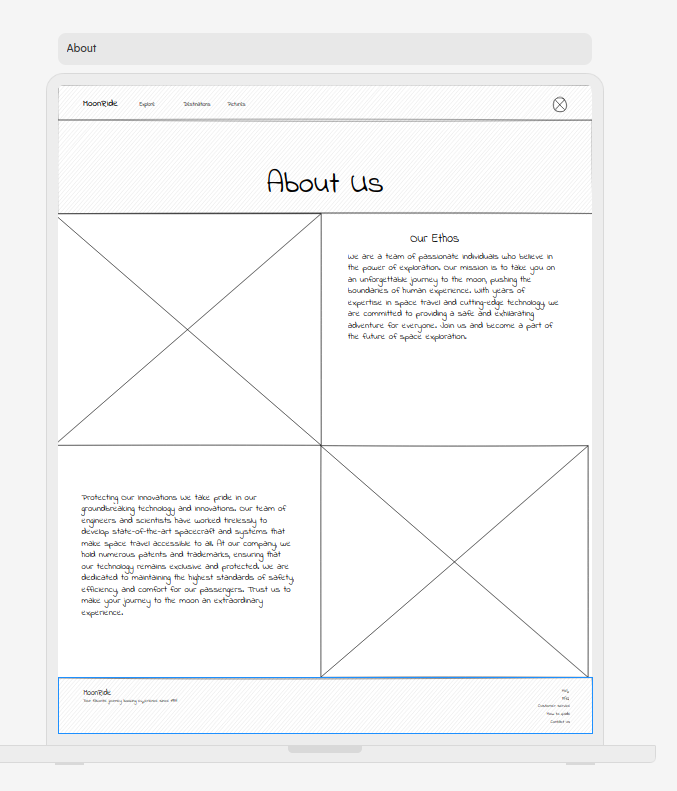
\includegraphics[width=0.45\linewidth]{AboutUs.png}
    \includegraphics[width=0.45\linewidth]{{AboutUsmedia.png}}
    \caption{The About Us page}
    \label{fig:AboutUsPage}
\end{figure}

The About Us page will detail the company's ethos, history, what is unique about their work, and information about key people behind the company. It is a static text and images page that the client can later edit.

\subsubsection{User Profile}
\begin{figure}[H]
    \includegraphics[width=0.45\linewidth]{{Profile.png}}
    \includegraphics[width=0.45\linewidth]{{ProfileMedia.png}}
    \caption{The Profile Page}
    \label{fig:ProfilePage}
\end{figure}

The User Profile page will allow users to control their personal details stored on the site. It will be a modern styled page with grouped settings on the left, more specific settings for each group in the middle and the customers bookings on the right.
\pagebreak
\appendix

\section{Appendix Client Questionnaire}

Q: Can you describe your brand?
\\
\\
Client: Our company brand for The Great UNKNOWN is a company that can expand the consciousness of the human race by taking people into space to experience the expanse and glory of space. We are a small start up and with that we want to take small steps into the outer reaches of adventure by initially taking people to the moon and back. 
\\
\\
Q: Can you give us an outline of your project?
\\
\\
Client: We want a simple website that will inform people about outer space and entice them into wanting to take on their biggest adventure. 
The website should consist of six pages: a homepage; customer login/join page; book your journey; about us; pictures of use; and user account management page
\\
\\
Q: What should be on the homepage?
\\
\\
Client: The homepage is the first page that our customers will see when the open the website it must include pictures of the previous voyagers and advances in our space technology. Text will be interleaved between the photos or on top of the pictures to show why customers should spend their money on a trip with us. There should be a static navbar with links to the other pages on the site and also a footer with a navbar with links to other information e.g. financial reports, history, Terms of Service (ToS) etc
\\
\\
Q: What should be in the login page?
\\
\\
Client:  The Login Page must be simple and straightforward. It should contain a box with a username, password and name and a sign up login button. After the customer has logged in they will be requested to add their billing address and bank details. When they have completed the setup they will be redirected to the Book Your Journey page.
\\
\\
Q: What will be in the User Account Management Page?
\\
\\
Client: The User Account Management Page (U.A.M) has to include a section to allow the customer’s billing address, bank details, password and usernames to be amended and their account deleted
\\
\\
Q: What should be on the Book Your Journey page?
\\
\\
Client: This page should be seamless for the user. When they open the page they will be immediately presented with a list of journeys that are currently available. The page will include a table which will be organised as a calendar, the month will be shown at the top and below that to the left will be the days. Time slots will be included to the right, with small red dots in the middle indicating availability. 
\\
\\
Q: What is the Pictures of Us page?
\\
\\
Client: The Pictures page should be minimalist in design little so no words will be included just what is necessary to describe the what the image is showing. The layout of the page will have one image going after another in a square like pattern, where the box's can vary in size depending on important the image is or what size the image is. By showing these images it will hopefully entice the user to be apart of our journey together and see the what is beyond our small plant that we call home.
\\
\\
Q: What is in the About us page?
\\
\\
Client: The About Us page should include all the legal documents showing the necessary certificates that prove we are certified to fly these ships. It will explain our ethos, who we are and why we want to take customers in to space. It should detail all copyrights, trademarks and patents so no one can
copy our ships and steal our designs.
\\
\\
Q: What is your Target Market?
\\
\\
Client: Our target market is people who can afford to go in to outerspace and who also want to be a part of unique and special experience that few people will have ever been able to take part in. They need to be adventurous, have an open heart and also be fit enough to be able to withstand the rigours of space travel.
\\
\\
Q: Who are you competitors?
\\
\\
Client: Currently our competitors are Space X, Blue Origin and NASA
\\
\\
Q: Do you have a budget?
\\
\\
Client: One Billion Dollars
\\
\\
\\
This a mocked up wireframe based on the requirements after the first draft before it was shown to the client https://app.uizard.io/p/302e3b62



\end{document}